\begin{figure}[htbp]
\centering
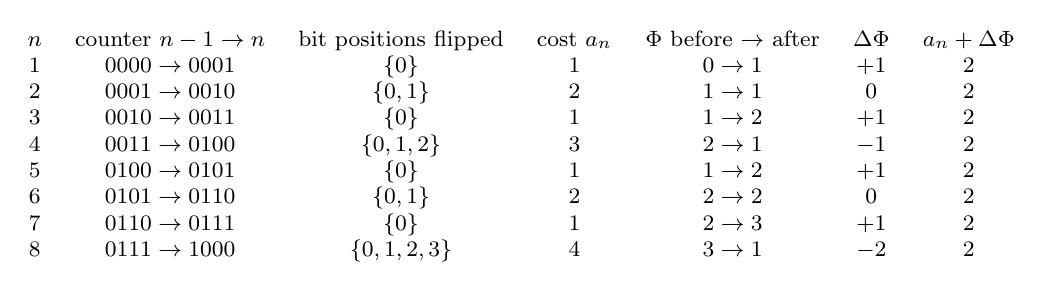
\begin{tikzpicture}
  \node[inner sep=0pt] {\footnotesize
    \begin{tabular}{@{}c c c c c c c@{}}
      \toprule
      $n$ & counter $n-1\to n$ & bit positions flipped & cost $a_n$ & $\Phi$ before $\to$ after & $\Delta\Phi$ & $a_n+\Delta\Phi$ \\
      \midrule
      $1$ & $0000\to0001$ & $\{0\}$       & $1$ & $0\to1$ & $+1$ & $2$ \\
      $2$ & $0001\to0010$ & $\{0,1\}$     & $2$ & $1\to1$ & $0$  & $2$ \\
      $3$ & $0010\to0011$ & $\{0\}$       & $1$ & $1\to2$ & $+1$ & $2$ \\
      $4$ & $0011\to0100$ & $\{0,1,2\}$   & $3$ & $2\to1$ & $-1$ & $2$ \\
      $5$ & $0100\to0101$ & $\{0\}$       & $1$ & $1\to2$ & $+1$ & $2$ \\
      $6$ & $0101\to0110$ & $\{0,1\}$     & $2$ & $2\to2$ & $0$  & $2$ \\
      $7$ & $0110\to0111$ & $\{0\}$       & $1$ & $2\to3$ & $+1$ & $2$ \\
      $8$ & $0111\to1000$ & $\{0,1,2,3\}$ & $4$ & $3\to1$ & $-2$ & $2$ \\
      \bottomrule
    \end{tabular}};
\end{tikzpicture}
\caption{Eight increments from zero, with bit positions numbered from the least significant bit. The displayed potential is the number of $1$ bits.}
\label{fig:counter}
\end{figure}
